\documentclass[handout, 10pt]{beamer}

%\usepackage[backend=bibtex,firstinits=true,style=verbose-inote,citestyle=authortitle]{biblatex}
\usepackage{bm}
\usepackage{graphicx}
\usepackage{subcaption}
\usepackage{amsmath}
\usepackage{amsfonts}
\usepackage{makecell}
\usepackage{filecontents}
\usepackage{biblatex}
\usepackage{xcolor}
\usepackage{subcaption}
% \newcommand{\expect}[2][]{
\ifthenelse{\equal{#1}{}}{
\mathbb{E}\left[#2\right]
}{
\underset{#1}{\mathbb{E}}\left[#2\right]
}}

\newcommand{\cov}[2][]{
\ifthenelse{\equal{#1}{}}{
\text{Cov}\left[#2\right]
}{
\underset{#1}{\text{Cov}}\left[#2\right]
}}


\newcommand{\var}[2][]{
\ifthenelse{\equal{#1}{}}{
\text{Var}[#2]
}{
\underset{#1}{\text{Var}}[#2]
}}

\newcommand{\loss}[2][]{
\ifthenelse{\equal{#1}{}}{
\mathcal{L}(#2)
}{
\mathcal{L}_{#1}(#2)
}}

\newcommand{\kl}[2]{
\text{D}_\text{KL}[#1 \parallel #2]
}

\newcommand{\R}{\mathbb{R}}
%\newcommand{\Prob}{\mathbb{P}}

\newcommand{\1}[1]{\mathds{1}\{#1\}}


%\usecolortheme{dolphin}
\setbeamertemplate{navigation symbols}{}
\setbeamertemplate{section in toc}{\inserttocsectionnumber.~\inserttocsection}

\begin{filecontents*}{references.bib}
@misc{FourierINR,
    title={Fourier Features Let Networks Learn High Frequency Functions in Low Dimensional Domains},
    author={Matthew Tancik and Pratul P. Srinivasan and Ben Mildenhall and Sara Fridovich-Keil and Nithin Raghavan and Utkarsh Singhal and Ravi Ramamoorthi and Jonathan T. Barron and Ren Ng},
    year={2020},
    eprint={2006.10739},
    archivePrefix={arXiv},
    primaryClass={cs.CV}
}
\end{filecontents*}


\addbibresource{references.bib}


\title{Fourier Features Let Networks Learn High Frequency Functions in Low Dimensional Domains\footnote{\citepaper{FourierINR}}}
%\subtitle{}
%\author{Ivan Skorokhodov}
%\date{}
%\logo{
\includegraphics[height=1cm]{images/ipavlov-logo.png}}

\newcommand{\citepaper}[1]{\citetitle{#1} by \citeauthor{#1}, \citeyear{#1}}

%\graphicspath{{./images}}

%\usetheme{lucid}
\begin{document}

\begin{frame}
    \titlepage
\end{frame}

\begin{frame}{Overview if INRs}
    \begin{itemize}
        \item\pause Recently, there appeared a new paradigm of representing signals
        \item\pause One can represent images/3D-objects/video/audio/etc as \textit{implicit neural representations} (INR)
        \item\pause INR is a neural network $\Phi(v)$ which takes a coordinates vector $v$ and produces a pixel/voxel/frequency/etc value at that point:
        \begin{figure}
            \centering
            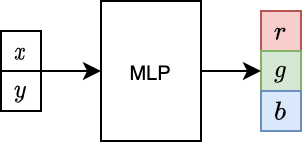
\includegraphics[width=0.4\textwidth]{images/inr}
            \caption{INR for 2D images: at each coordinate we predict a pixel value}
        \end{figure}
        \item\pause I.e. one neural network corresponds to a single image.
    \end{itemize}
\end{frame}

\begin{frame}{Overview of the paper}
\begin{itemize}
    \item\pause Authors showed that standard MLPs fail to learn high frequency functions (both in theory and in practice)
    \item\pause They showed that using ``fourier features'' overcomes the issue
    \item\pause They test their ideas on a range of INR tasks: reconstructing images/3D-shapes/MRI-images/etc
    \item\pause They used JAX to implement this all
\end{itemize}
\end{frame}

\begin{frame}{Intuition. Part 1/3: the foreword}
\begin{itemize}
    \item\pause Let's roughly divide images into low-frequency images and high-frequency images:
    \begin{itemize}
        \item\pause In a low-frequency image, things change slow from pixel to pixel
        \item\pause In a high-frequency image, things change fast
    \end{itemize}
    \begin{figure}
        \begin{subfigure}{0.45\textwidth}
            \centering
            
\includegraphics[width=0.9\linewidth]{images/sky}
            \caption{A low-frequency image}
        \end{subfigure}
        \begin{subfigure}{0.45\textwidth}
            \centering
            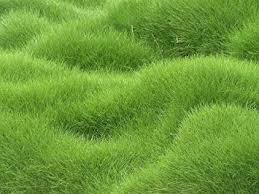
\includegraphics[width=0.9\linewidth]{images/grass}
            \caption{A high-frequency image}
        \end{subfigure}
    \end{figure}
\end{itemize}
\end{frame}

\begin{frame}{Intuition. Part 2/3: the problem}
\begin{itemize}
    \item\pause Neural networks are bad at distinguishing small values between each other
    \item\pause For example, if your input is 0.03 and you replace it with 0.05, your model will likely not to notice any difference
    \item\pause And this is the main cause of why MLPs fail to model high-frequency images:
    \begin{itemize}
        \item\pause Our input coordinates for an INR lie in $[0,1]$ domain
        \item\pause For high-frequency images, output changes a lot when an input changes slightly
        \item\pause Our model is incapable to detect small changes in the input
        \item\pause The result: MLPs "oversmooth" high-frequency images
    \end{itemize}
    \begin{figure}
        \centering
        \begin{subfigure}{0.45\textwidth}
            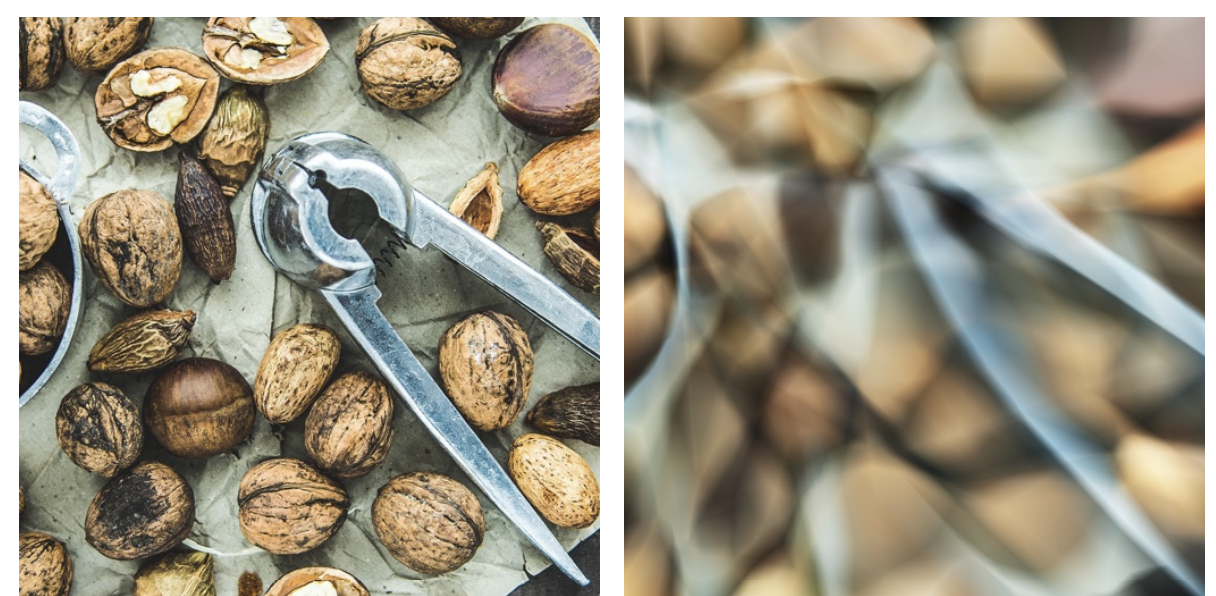
\includegraphics[width=0.9\textwidth]{images/mlp-oversmooth-nut}
        \end{subfigure}
        \begin{subfigure}{0.45\textwidth}
            \centering
            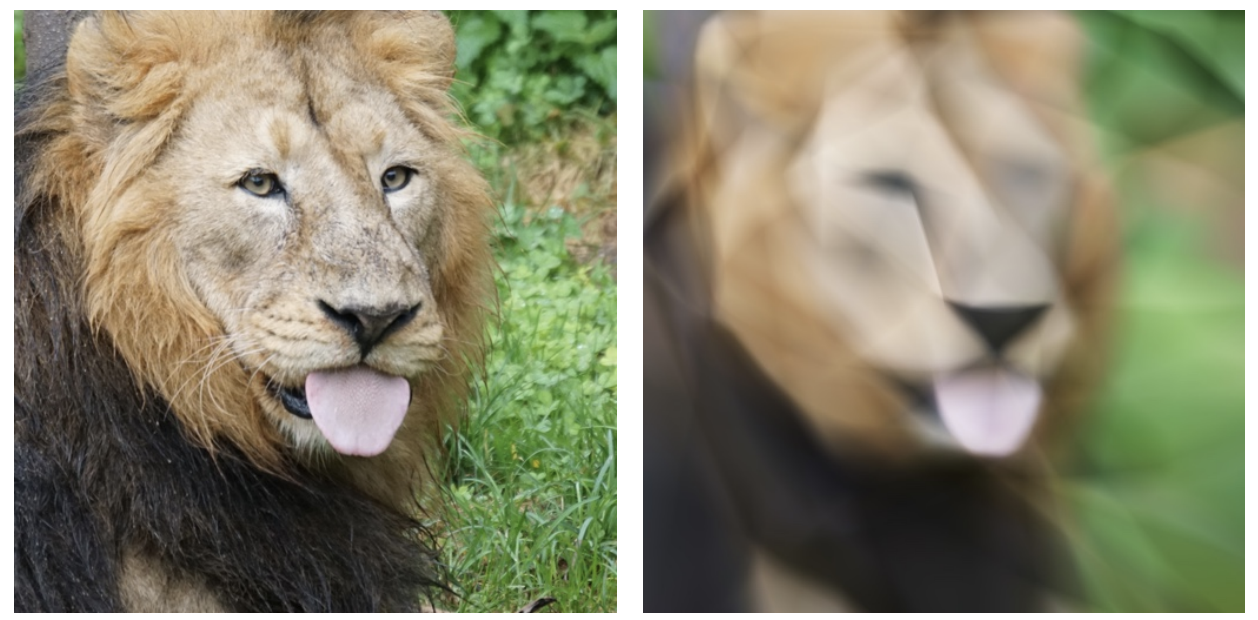
\includegraphics[width=0.9\textwidth]{images/mlp-oversmooth-lion}
        \end{subfigure}
        \caption{INR is trained to reconstruct an image: MLP oversmoothes high-frequency images}
    \end{figure}
\end{itemize}
\end{frame}

\begin{frame}{Intuition. Part 3/3: the solution}
\begin{itemize}
    \item\pause How can we help the model to detect small changes in an input?
    \begin{itemize}
        \item\pause Step 1: multiply by a very large number
        \item\pause Step 2: apply $sin(x)$ or $cos(x)$
    \end{itemize}
    \begin{figure}
        \centering
        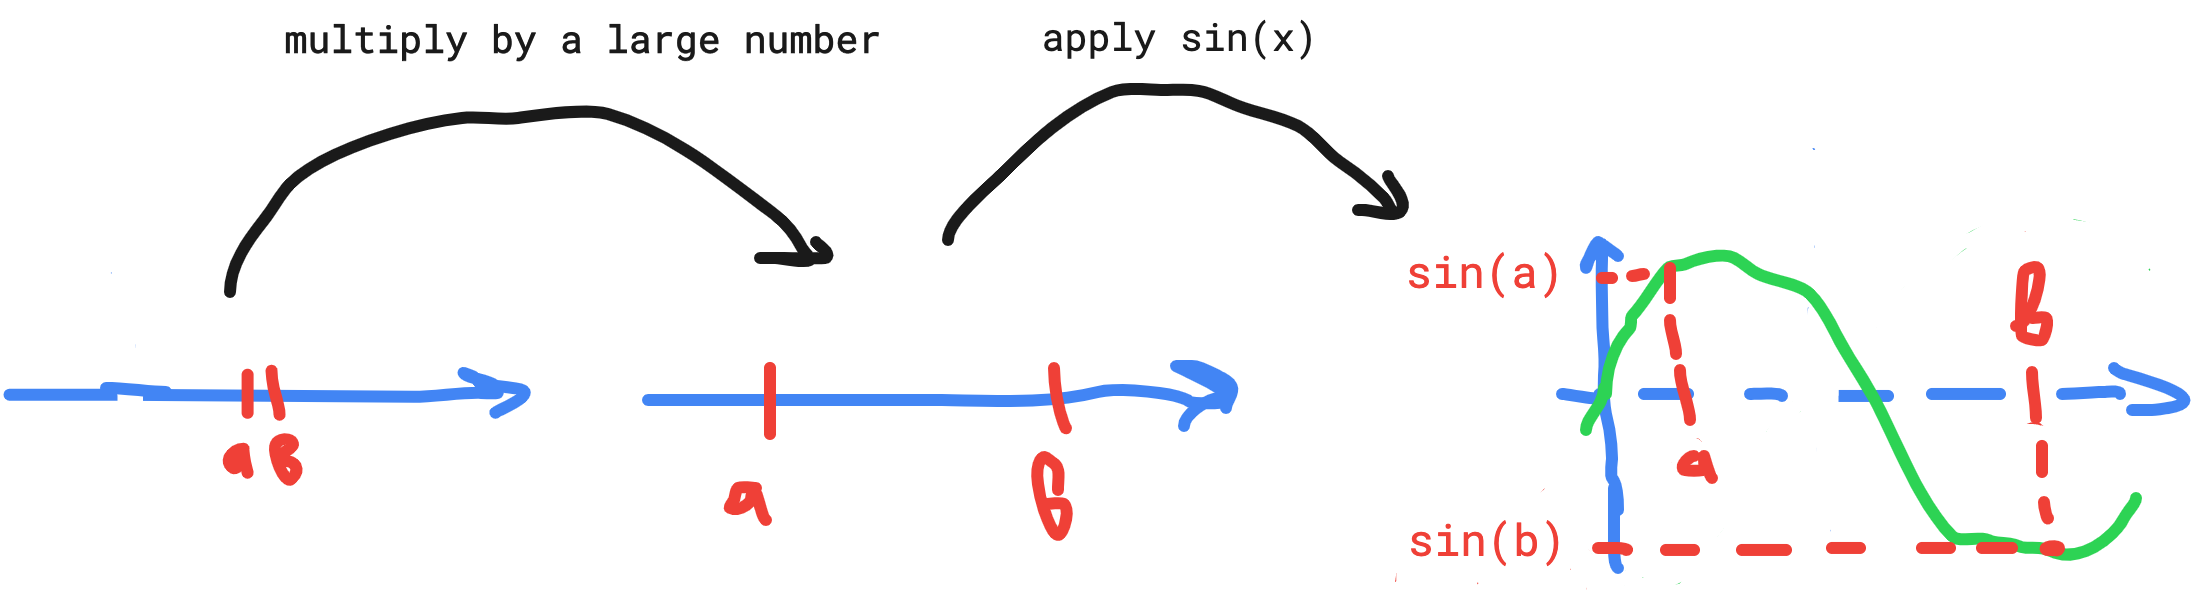
\includegraphics[width=\textwidth]{images/intuition-illustration}
        \caption{Intuition of the positional encoding trick}
    \end{figure}

    \item\pause Why do we need sines/cosines?
    \begin{itemize}
        \item\pause Neural networks do not like large-magnitude values (due to exploding variance)
        \item\pause Authors also show that this allows a model to have a shift-invariance property
    \end{itemize}
\end{itemize}
\end{frame}

\begin{frame}{Kernel regression}
\begin{itemize}
%    \item\pause INRs solve a regression task: given coordinates, predict a value in the interval $[0,1]$
    \item\pause Kernel regression is the following machine learning algorithm:
    \begin{itemize}
        \item\pause Obtain a training dataset $\bm X, \bm y$
        \item\pause Obtain a kernel function $k(\bm x,\bm x')$ (it's like a similarity function)
        \item\pause Compute kernel matrix $\bm K$ where $K_{ij} = k(\bm x_i, \bm x_j)$
        \item\pause Compute the value for a test point $\bm x$ by:
        \begin{equation}
\hat{f}(\mathbf{x})=\sum_{i=1}^{n}\left(\mathbf{K}^{-1} \mathbf{y}\right)_{i} k\left(\mathbf{x}_{i}, \mathbf{x}\right)
\end{equation}
    \end{itemize}
\end{itemize}
\end{frame}

\begin{frame}{NTK theory}
NTK (Neural Tangent Kernel) theory explores the behaviour of infinite-width MLPs:
\begin{itemize}
    \item\pause If the learning rate is small then the MLP simplifies to kernel regression with:
\begin{equation*}
k_{\mathrm{NTK}}\left(\mathbf{x}_{i}, \mathbf{x}_{j}\right)=\mathbb{E}_{\theta \sim \mathcal{N}}\left\langle\frac{\partial f\left(\mathbf{x}_{i} ; \theta\right)}{\partial \theta}, \frac{\partial f\left(\mathbf{x}_{j} ; \theta\right)}{\partial \theta}\right\rangle
\end{equation*}
    \item\pause Matrix $\bm K$ is poorly conditioned for a regular MLP, i.e. it has few large eigenvalues and others are small
    \item\pause NTK shows that the components of the target function that correspond to large eigenvalues are learned much faster
    \item\pause Components with large eigenvalues have lower frequency
    \item\pause This makes the learning of high-frequency patterns too slow
    \item\pause Authors propose to preprocess input coordinates with Fourier mapping:
    \begin{itemize}
        \item\pause This would make $k_\text{NTK}$ be better conditioned
        \item\pause This would make $k_\text{NTK}$ stationary\footnote{i.e. $k(\bm x, \bm x') = h(\bm x - \bm x')$ for some $h$} which gives invariance to shifts
    \end{itemize}
\end{itemize}
\end{frame}

\begin{frame}{Fourier mapping for INRs}
    \begin{itemize}
        \item\pause Authors propose to embed the coordinates with:
        \begin{equation*}
\gamma(\mathbf{v})=\left[\cos \left(2 \pi \mathbf{b}_{1}^{\mathrm{T}} \mathbf{v}\right), \sin \left(2 \pi \mathbf{b}_{1}^{\mathrm{T}} \mathbf{v}\right), \ldots, \cos \left(2 \pi \mathbf{b}_{m}^{\mathrm{T}} \mathbf{v}\right), \sin \left(2 \pi \mathbf{b}_{m}^{\mathrm{T}} \mathbf{v}\right)\right]^{\mathrm{T}}
\end{equation*}
        where $\bm b_i$ are random vectors of size $d$ (for images, $d=2$)
        \item\pause This makes the NTK kernel stationary and have a better spectrum
        \item\pause Authors sample $\bm b_i$ from $\mathcal{N}(0, \sigma^2)$ where $\sigma^2$ is a large number
        \begin{figure}
            \centering
            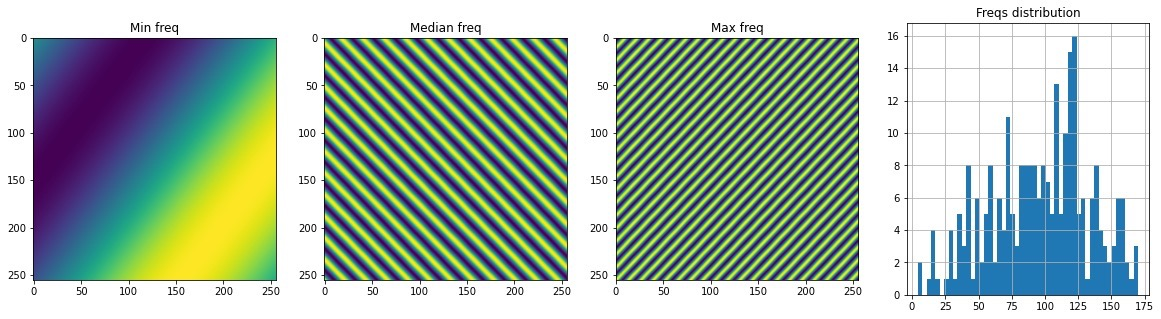
\includegraphics[width=\textwidth]{images/embedding-example}
            \caption{Visualization of the embeddings for some of the vectors $\bm b_i$ for $256 \times 256$ coordinates. Vectors $\bm b_i$ are sampled from uniform distribution.}
        \end{figure}
    \end{itemize}
\end{frame}

\begin{frame}{Results}
    \begin{figure}
        \centering
        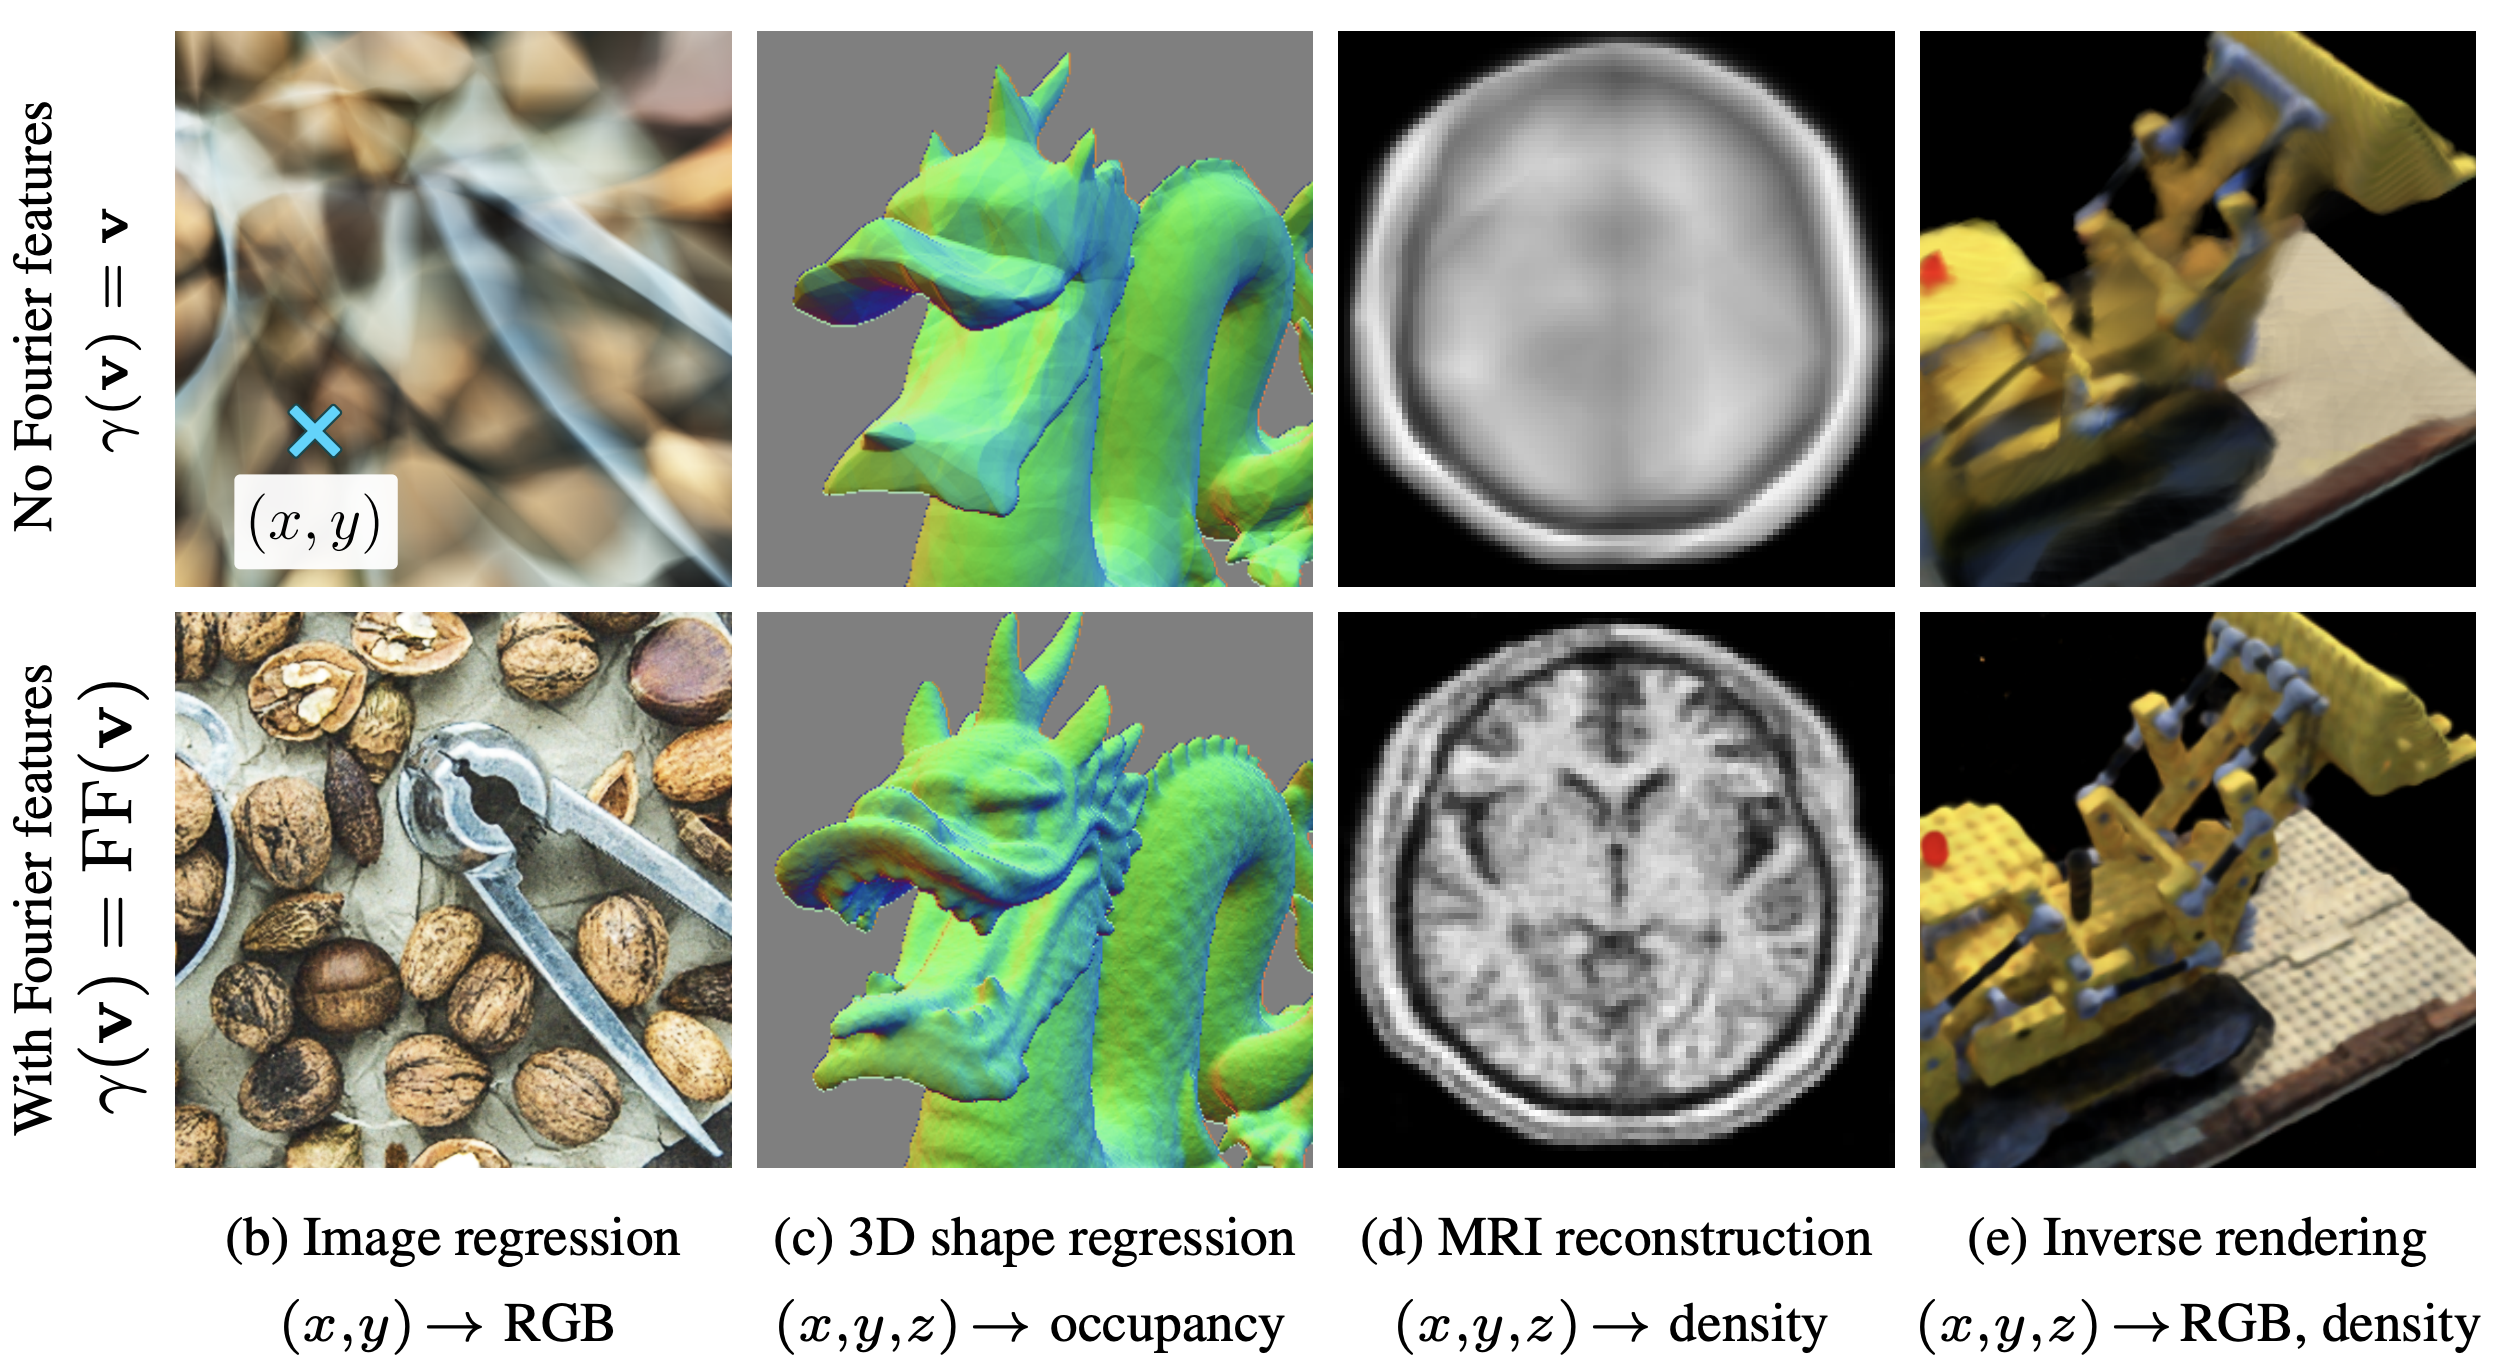
\includegraphics[width=0.9\textwidth]{images/results}
    \end{figure}
\end{frame}

\begin{frame}{Conclusion}
\begin{itemize}
    \item\pause Authors provide an interesting (but not very transparent) theoretical analysis of INRs
    \item\pause Their theoretical claims are confirmed by empirical evidence
    \item\pause They achieve strong results on several domains
    \item\pause One needs to search for optimal $\sigma$ value when sampling $\bm b$ from $\mathcal{N}(0, \sigma^2)$
\end{itemize}    
\end{frame}

\end{document}
